% example, page 03: a matrix product state -- arrays A on a chain, bonds between
% them (plain lines, the bond dimension D), occupation indices n_i down. A finite
% basis throughout, so no wavy legs. The fourth slot is the dots of a chain that
% goes on.
\documentclass[border=4pt]{standalone}
\input{preamble}
\usepackage{tikz-tensors}
\input{notation}

\begin{document}
\begin{tikzpicture}
  \tnstack{P}{5}{ket}
  \tnlayer{P}{ket}{3*coef/$A$, dots, coef/$A$}
  \tnconnect{P}
  \tnopen[labels={$n_1$, $n_2$, $n_3$, $n_N$}]{down}{P}
  \tnmid{P-ket-1}{P-ket-2}{$D$}
\end{tikzpicture}
\end{document}
